\chapter{Setup}

\section{Unpacking and Connecting the MEGA65}
\label{cha:setup}

It is time to set up your MEGA65 home computer! The box contains the following:

\begin{itemize}
\setlength\itemsep{-0.75mm}
\item MEGA65 computer
\item Power supply (black box with socket for mains supply)
\item This book, the MEGA65 User's Guide
\item Your personal registration code, on a piece of paper (possibly tucked into the User's Guide)
\end{itemize}

In addition, to be able to use your MEGA65 computer you will need:

\begin{itemize}
\item A television or computer monitor with a VGA or digital video input, capable of displaying an image at 480p (720x480) at 60Hz or 576p (720x576) at 50Hz
\item An appropriate video cable for your display, either VGA or digital video
\end{itemize}

You may also like to use the following to get the most out of your MEGA65:

\begin{itemize}
\item A digital video display with built-in audio, or powered speakers and an appropriate audio cable with 3.5mm audio jack connector
\item A microSD card, type SDHC, between 4GB and 32GB in size
\item An RJ45 Ethernet cable and a network router or switch
\item A fresh CR2032 battery, for the Real-Time Clock
\item A Phillips-head screwdriver, to access the inside of the case
\item A joystick or gamepad compatible with Commodore computers, with a nine-pin (DE-9) connector\index{Joystick}
\item A Commodore 1351 mouse, an Amiga mouse, or a modern replacement such as a \href{https://retrohax.net/shop/amiga/mouster/}{mouSTer} USB mouse adapter\index{Commodore 1351 mouse}\index{Commodore Amiga mouse}\index{mouSTer adapter}
\end{itemize}

\newpage
\section{Rear Connections}
\index{Case!Connections}

\includegraphics[width=\linewidth]{images/illustrations/mega65-rear.pdf}
\begin{center}
\setlength{\def\arraystretch{1.5}\tabcolsep}{6pt}
\begin{longtable}{ c | l}
	1	& 	3.5mm Audio Jack \\
	2	& 	External microSD Card Slot\\
	3	& 	Network LAN Port \\
	4	& 	Digital Video Connector (including sound) \\
	5	& 	VGA Video Connector \\
	6	& 	IEC Serial Bus Connector for Disk Drives and Printers \\
	7	& 	Cartridge Expansion Port \\
	8	& 	Power Supply Socket \\
\end{longtable}
\end{center}

%\newpage
\vspace{-1cm}

\section{Side Connections}

\includegraphics[width=\linewidth]{images/illustrations/mega65-side.pdf}

\begin{center}
\setlength{\def\arraystretch{1.5}\tabcolsep}{6pt}
\begin{longtable}{ c | l}
	1	& 	Power Switch \\
	2	& 	Controller Port 2 \\
	3	& 	Controller Port 1 \\
	4	& 	Reset Button \\
\end{longtable}
\end{center}

Various peripherals can be connected to Controller Ports 1 and 2 such as
joysticks, paddles or mouse devices.

\newpage

\section{MEGA65 Screen and Peripherals}

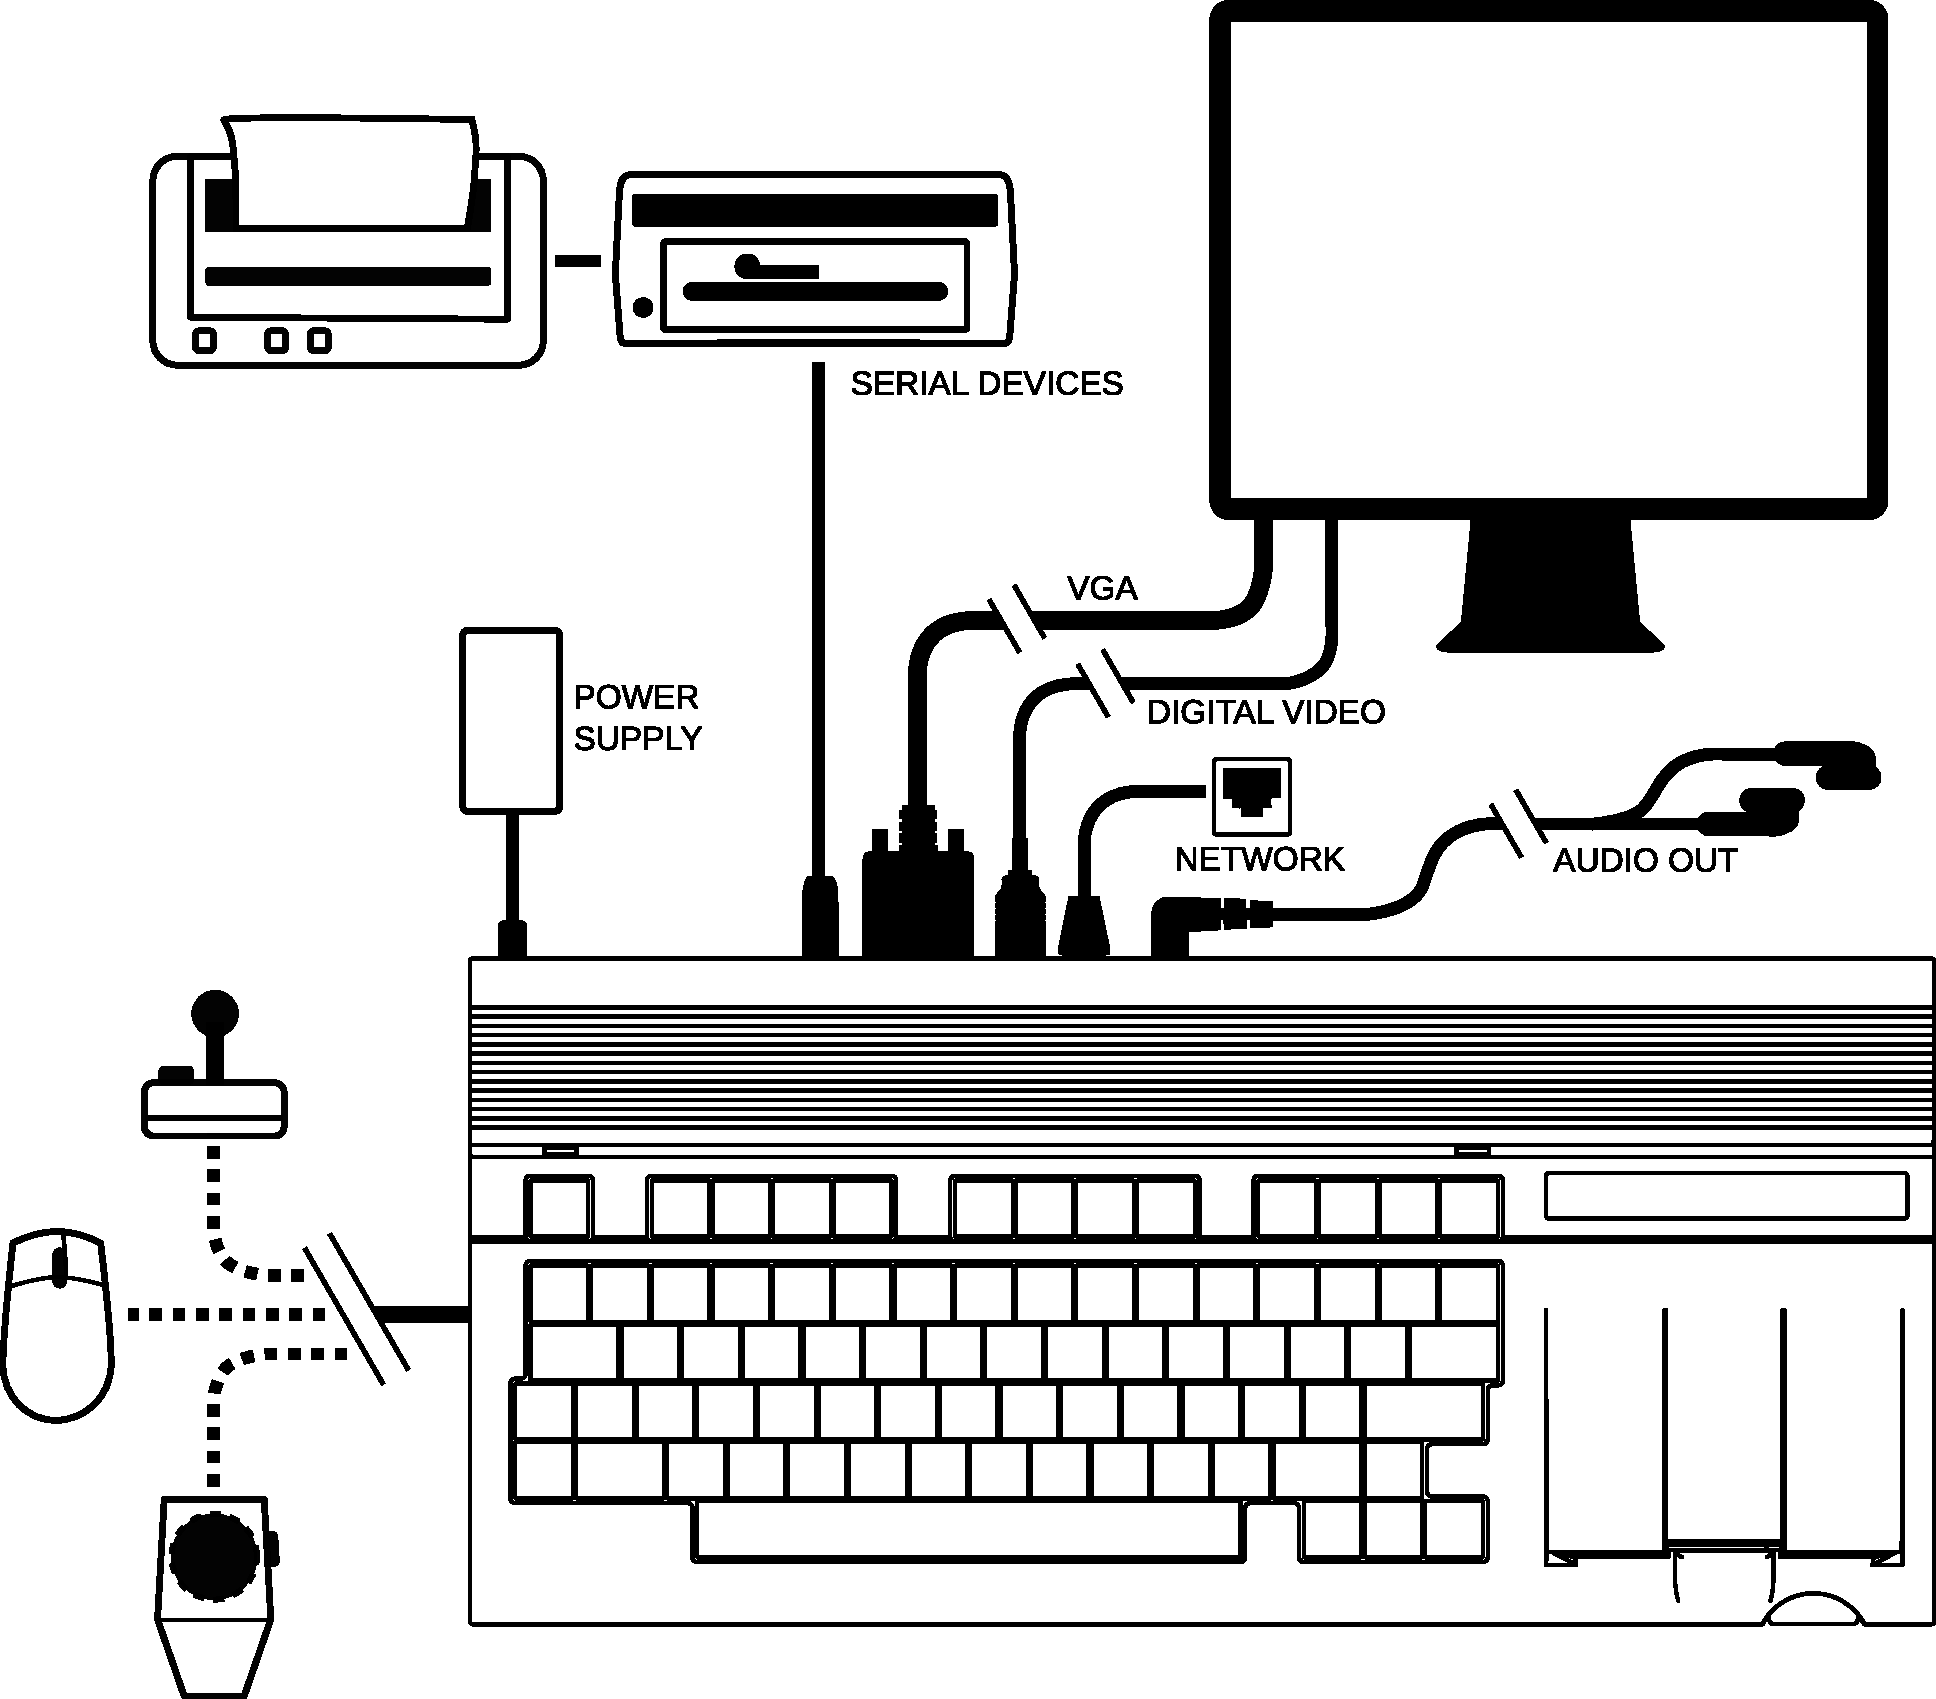
\includegraphics[width=\linewidth]{images/illustrations/mega65-top.pdf}

To connect your MEGA65 to a display:
\index{Display!Connecting}

\begin{enumerate}
	\item Connect the power supply to the power supply socket of the MEGA65.
	\item If you have a VGA monitor and a VGA cable, connect one end to the VGA port of the MEGA65 and the other end into your VGA monitor.
	\item If you have a TV or monitor with a compatible Digital Video connector,\footnote{The Digital Video connector type has a recognizable four-letter commercial name, but the MEGA65 project has not paid the licensing fees to refer to it by this name. This {\em User's Guide} refers to this as the ``Digital Video'' connector.}\index{Digital Video} connect one end of your cable to the Digital Video port of the MEGA65, and the other into the Digital Video port of your monitor. If you own a monitor with a DVI socket, you can use a Digital Video to DVI adapter.
\end{enumerate}

\newpage
\section{Optional Connections}
\index{Disk Drives!Connecting}
\index{Connections!IEC}
\index{SD Cards!Locations}
\begin{enumerate}
	\item The MEGA65 includes an internal 3.5" floppy disk drive. You can also connect older Commodore{\textregistered} IEC serial floppy drives to the MEGA65, such as the Commodore 1541, 1571 or 1581. To use these drives, connect one end of an IEC cable to the Commodore floppy disk drive and the other end to the Disk Drive socket of the MEGA65. You can also connect an SD2IEC device\index{SD2IEC device} or a Pi1541 device.\index{Pi1541 device} With most devices, you can daisy-chain additional floppy disk drives or Commodore compatible printers.
	\item You can connect your MEGA65 to an Ethernet network using a standard Ethernet cable.
	\item For enjoying audio from your MEGA65, you can connect a 3.5mm audio jack cable to an audio amplifier or speaker system. If your system has RCA connectors you will need a 3.5mm audio jack to twin RCA adapter cable. The MEGA65 also has a built-in amplifier to allow the use of headphones.
	\item A microSD card, type SDHC between 4GB and 32GB, can be inserted into the external microSD card slot at the rear of the MEGA65. For more information on using the microSD card slot, see ``Introducing SD Cards'' on page \pageref{sec:introducing-sd-cards}.
	\item Underneath the MEGA65, a small door provides access to the internal SD card and two connectors for future hardware expansion.
\end{enumerate}

\index{Real-Time Clock!Installing the Battery}
\subsection{Installing the Real-Time Clock Battery}

The MEGA65 includes a Real-Time Clock, which is used to display the time and date on the startup screen, to add timestamps to files that the MEGA65 writes to your SD cards, and by the {\bf DT\$}\index{BASIC 65 Variables!DT} and {\bf TI\$}\index{BASIC 65 Variables!TI\$} BASIC65 variables. This clock utilises a CR2032 coin-cell battery\footnote{Early models of MEGA65 with the "R3A" board revision used a battery of type CR1220 for the Real-Time Clock. Revisions "R5" and later, which began shipping in late 2023, use a CR2032 battery.} to keep time when the MEGA65 isn't switched on. The MEGA65 does not include a battery in order to avoid issues related to shipping batteries internationally.

To install the battery, use a Phillips-head screwdriver to open the case, exposing the motherboard.\index{Case!Opening} The case is held together with three screws, all of which are along the bottom of the front side of the case. Once the screws have been removed, carefully lift the top half of the case. Note the orientation of the keyboard connector, then disconnect it.

The battery is located between the controller ports and the keyboard connector.

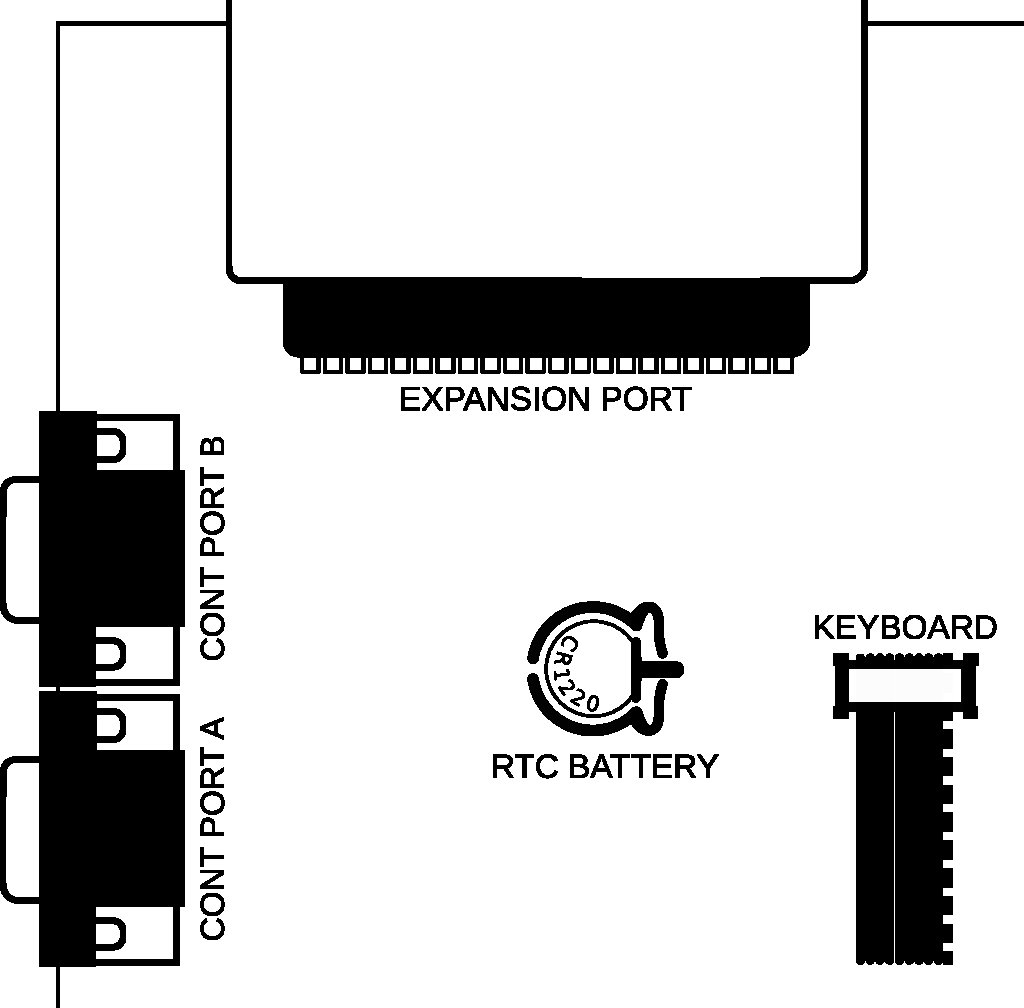
\includegraphics[width=\linewidth]{images/illustrations/rtc-battery-location.pdf}

If you are removing an existing battery, push the battery release lever on the bottom (flat-sided) side of the battery socket away from the battery to remove it. Insert the new battery with the side labelled {\bf +} facing up, and press it into place.

Once you have re-assembled your MEGA65, you can set the time in the Configuration Utility. For more information on how to set the Real-Time Clock, refer to the Configuration Utility section on page \pageref{sec:configuration-utility}.


\newpage

\section{Switching the MEGA65 on for the First Time}
\label{onboarding}

Switch the MEGA65 on using the power switch on the left-hand side of the computer.

When you switch your MEGA65 on for the first time, it displays the initial configuration (``on-boarding'') screen.\index{Configuration!On-boarding} You can use this screen to set the time and date on the Real-Time Clock (if you have installed the CR2032 battery), change the video display mode, and test the audio. All of these settings can be changed later.

\begin{center}
  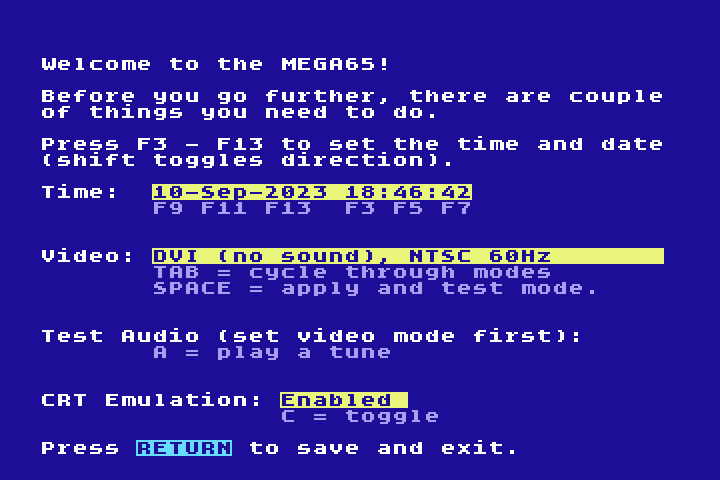
\includegraphics[width=0.7\linewidth]{images/img011_final_boot_01.png}
\end{center}

For video display modes, you can select between PAL\index{PAL display mode} or NTSC\index{NTSC display mode} emulation, and you can select whether your Digital Video display supports sound. If you are using the VGA video output, the Digital Video sound mode has no effect.

\underline{Note}: A DVI display that does not support sound will not work with the ``enhanced'' sound mode. With such a display, you must select a video mode with ``no sound,'' and connect a speaker to the 3.5 mm audio jack.

PAL and NTSC are analog video signal formats that affect the resolution and vertical sync speed of the video output, even when using a modern digital display. Your display may support either mode, or it may only support one or the other. You can use this screen to test the modes with your display.

Select and test your video configuration. For example, press \specialkey{TAB} to switch to the {\bf PAL 50HZ} mode.
\index{Display!Setting PAL/NTSC}
\begin{center}
  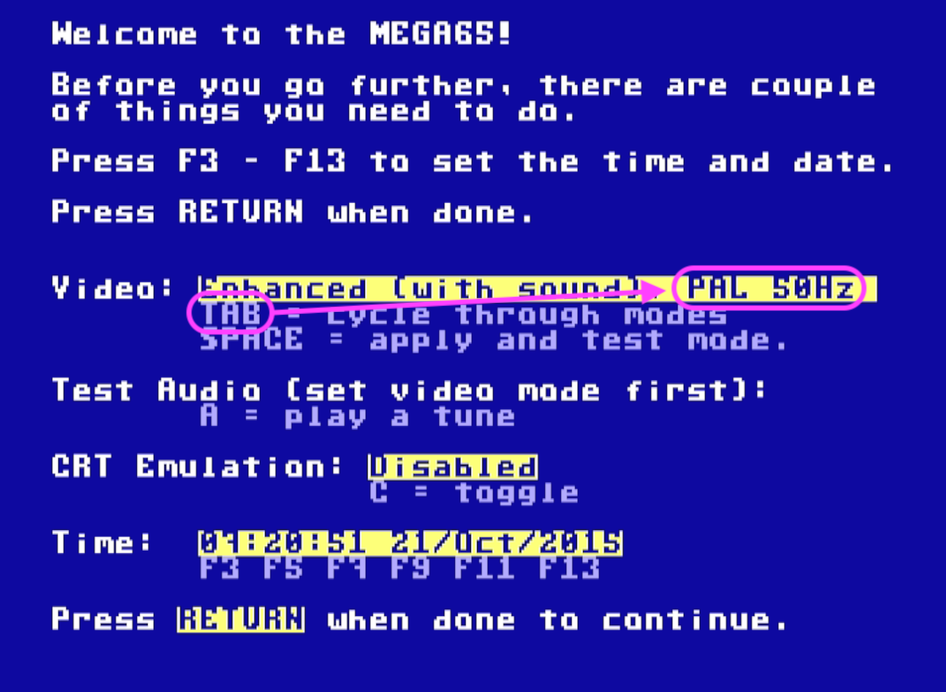
\includegraphics[width=0.7\linewidth]{images/img011_final_boot_02.png}
\end{center}

Press \megakey{SPACE} followed by \megakey{Y} to test the new video mode.

\begin{center}
  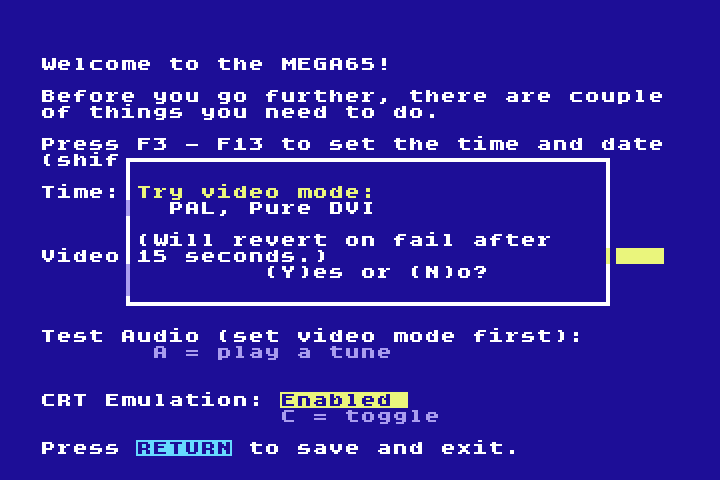
\includegraphics[width=0.7\linewidth]{images/img011_final_boot_03.png}
\end{center}

Press \megakey{K} to keep the new video mode.

\begin{center}
  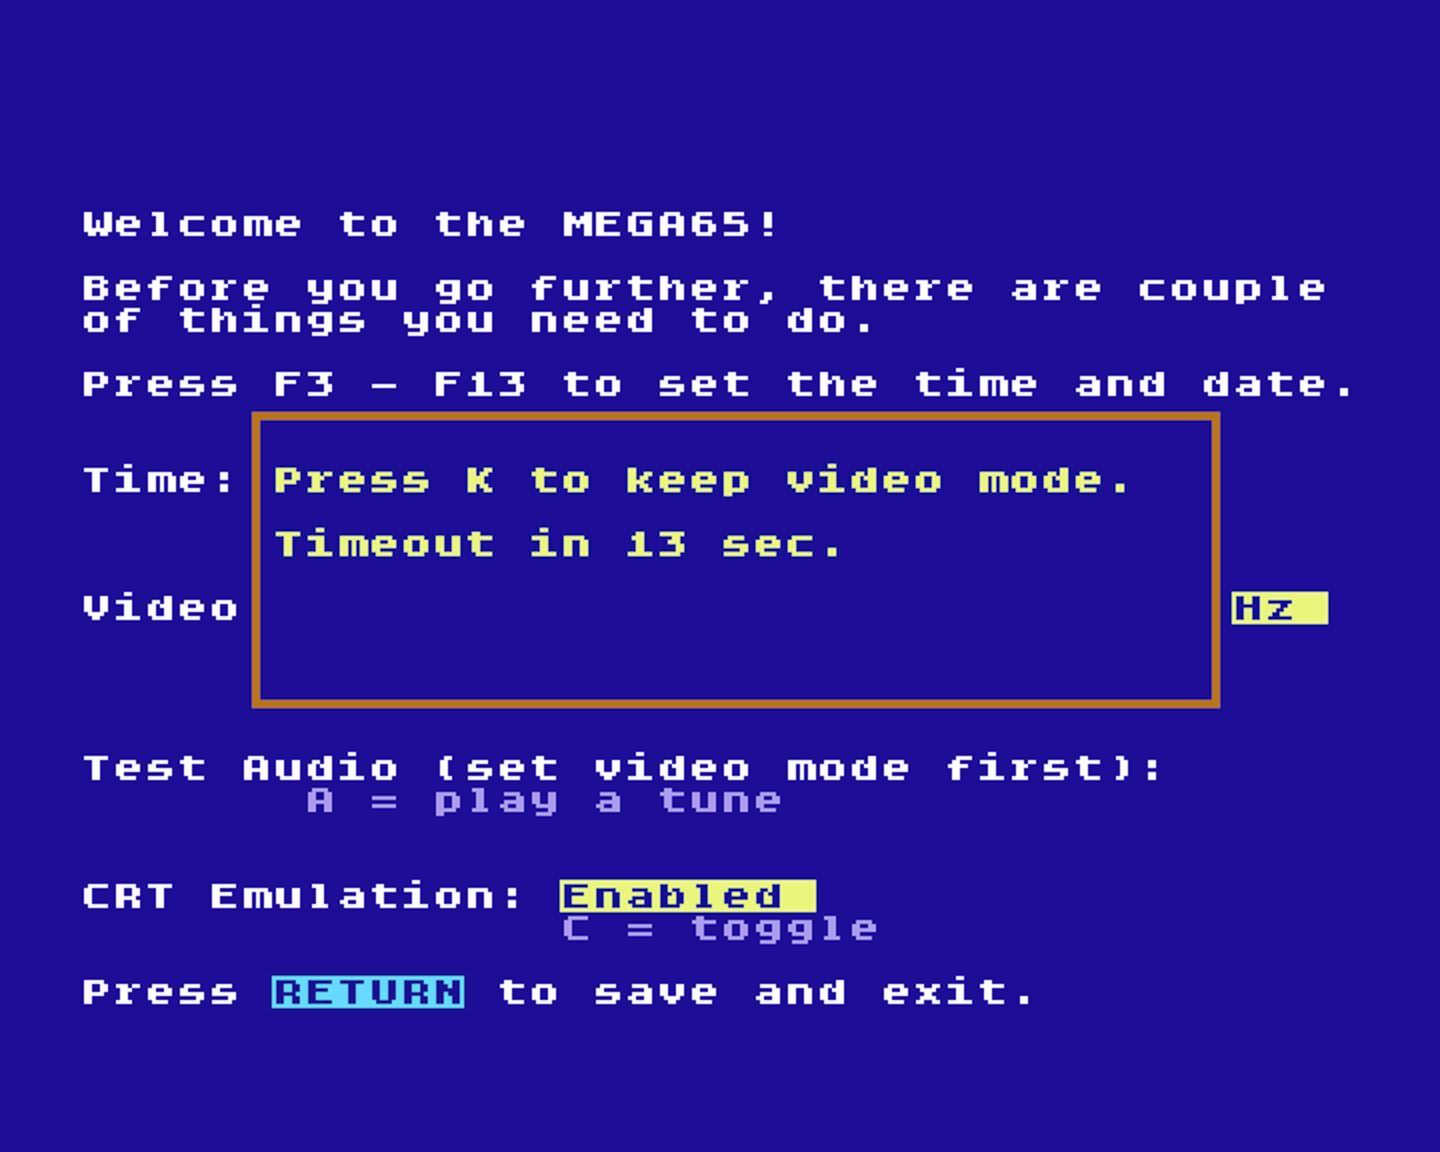
\includegraphics[width=0.7\linewidth]{images/img011_final_boot_04.png}
\end{center}

Take this opportunity to test your sound set-up. Press \megakey{A} to play a sound.

The ``CRT emulation'' option is a fun choice when using a modern flat panel display. It adds vertical gaps between pixels to simulate the CRT raster line. Try it to see if you like it: press the \megakey{C} key to toggle it on and off.

Finally, press \specialkey{RETURN} to complete the configuration.

For more information about configuring your MEGA65, see chapter \vref{cha:configuringyourmega}.

\section{The Intro Disk}
\index{Intro Disk}

After completing the on-boarding configuration, your MEGA65 starts the Intro Disk menu. The Intro Disk is a collection of software made by the MEGA65 community that demonstrates some of the capabilities of the computer. Take some time to browse the menus and try some of the demos. After each demo, press the reset button on the left-hand side of the computer to return to the Intro Disk menu.

\begin{center}
  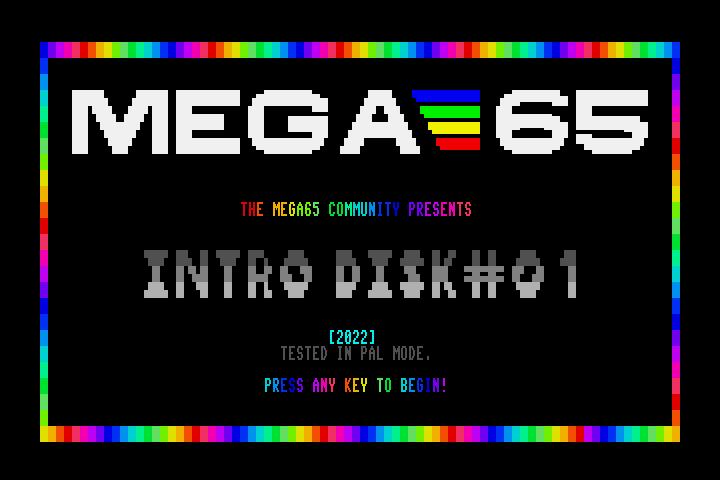
\includegraphics[width=0.7\linewidth]{images/demo_title.png}
\end{center}

By default, the Intro Disk menu opens each time you switch on the computer. Once you are more familiar with the MEGA65, you may wish to disable this. Press \megakey{D} at the Intro Disk menu to disable its auto-boot feature.\index{Intro Disk!Disabling}

Press \megakey{X} to exit the Intro Disk menu and access BASIC 65. With the Intro Disk auto-boot feature disabled, the MEGA65 goes directly to BASIC 65 when you switch it on.

\begin{center}
  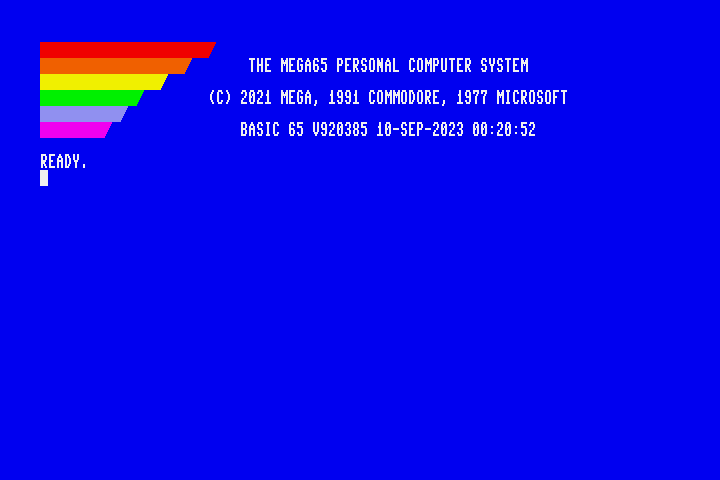
\includegraphics[width=0.7\linewidth]{images/img011_final_boot_06.png}
\end{center}

\section{The Cursor}

The flashing square underneath the \screentext{READY} prompt\index{READY prompt} is called the cursor. The cursor indicates that the computer is ready to accept input. Pressing keys on the keyboard will print their respective characters onto the screen. The characters will be printed at the current cursor position, and the cursor will advance to the next position after every key press.

Here you can type commands, that can do things such as loading a program. You can also start entering program code!
